% ECE4900W Communicating Engineering Solutions
% Author: Arturo Salinas-Aguayo <artjsalina5@uconn.edu>
\documentclass{beamer}
\setbeameroption{show notes}
\usetheme{Warsaw}
\usecolortheme{dolphin}
\usefonttheme{professionalfonts}
\setbeamertemplate{navigation symbols}{}
\usepackage{graphicx}
\usepackage{biblatex}
\addbibresource{references.bib}
\graphicspath{{../../images/}}

\title[Safe Nuclear Power]{Safe Nuclear Power: Instrumentation, Human Oversight, and Infrastructure Transition}
\subtitle{ECE 4900W – Summer 2025}
\author[Arturo Salinas]{Arturo Salinas-Aguayo}
\institute[UConn]{University of Connecticut\\College of Engineering}
\date{\today}

\begin{document}

\begin{frame}
  \titlepage
  \note{Welcome. This presentation explores the technological, ethical, and infrastructural dimensions of nuclear power in the modern world. We will cover lessons from historic accidents, instrumentation, human-machine interface design, and current innovations. Each story reveals both vulnerability and resilience.}
\end{frame}

\begin{frame}{Outline}
  \tableofcontents
  \note{Here is the roadmap for this presentation. Each section builds on the last, culminating in a call for renewed responsibility and innovation in the nuclear field.}
\end{frame}

\section{Introduction}
\begin{frame}
  \centering
  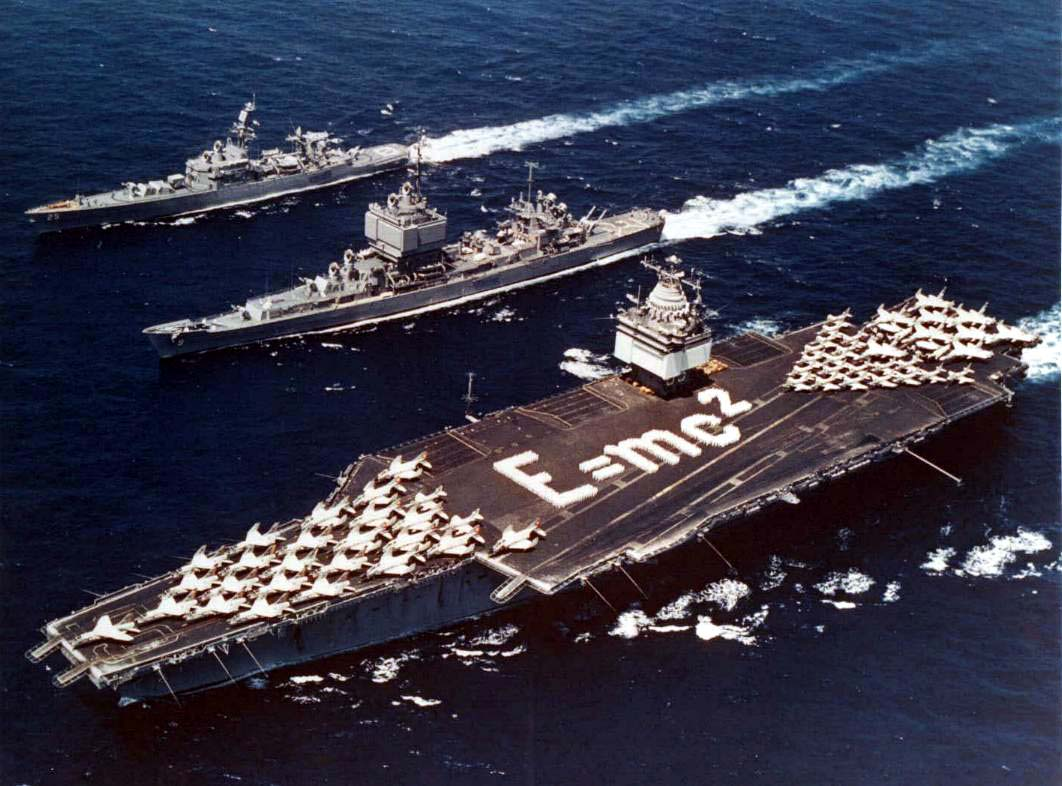
\includegraphics[width=\textwidth]{enterprise}
  \notes{i've been hearing a lot of misunderstanding when it comes to this epic photograph taken on july 31, 1964 with the uss enterprise, the uss long island, and the uss bainbridge. e = mc^2 refers to the fact that as the mass of the fuel increases, the potential for it to create energy is proprotional with that multiplied times the speed of light squared. the us navy was a big push for nuclear power and the enterprise alone had 8 submarine reactors powering her.}
\end{frame}
\begin{frame}{Motivation}
  \subsubsection*{Why Nuclear Now?}
  \begin{itemize}
    \item High energy density and steady base-load power
    \item Nearly zero emissions, independent of weather
    \item Risks of failure—catastrophic if unmanaged
  \end{itemize}
  \notes{Despite fears, nuclear remains one of the most efficient and clean energy sources. But it requires precision and care at every level.}
\end{frame}

\begin{frame}{The Fission Process}
  \subsubsection*{Where It All Begins}
  \begin{equation}
    ^{235}\text{U} + ^{1}\text{n} \rightarrow ^{92}\text{Kr} + ^{141}\text{Ba} + 3^{1}\text{n} + \text{Energy} \approx 200~\text{MeV}
  \end{equation}
  \begin{itemize}
    \item A neutron collides with uranium-235, causing it to split
    \item Releases energy and more neutrons → possible chain reaction
  \end{itemize}
  \note{This is the reaction that drives nuclear power. The energy release is immense, but so is the potential for instability if left uncontrolled.}
\end{frame}

\begin{frame}{Reactivity and Control}
  \subsubsection*{Choreographing Neutrons}
  \begin{equation}
    \rho = \frac{k_{\text{eff}} - 1}{k_{\text{eff}}}
  \end{equation}
  \begin{itemize}
    \item $k_{\text{eff}}$: effective neutron multiplication factor
    \item $\rho > 0$: supercritical (power increases)
    \item $\rho = 0$: critical (steady power)
    \item $\rho < 0$: subcritical (power decreases)
  \end{itemize}
  \note{Instrumentation exists to measure and control reactivity—avoiding runaway reactions like those at SL-1 and Chernobyl.}
\end{frame}

\section{Reactor Designs and Sensors}

\begin{frame}{Types of Reactors}
  \begin{itemize}
    \item Pressurized Water Reactor (PWR)
    \item Boiling Water Reactor (BWR)
    \item Heavy Water Reactor (CANDU)
    \item Advanced Gas-cooled Reactor (AGR)
  \end{itemize}
  \note{Each design uses different coolants and moderators, which affect safety logic and monitoring strategies.}
\end{frame}

\begin{frame}{PWR Instrumentation}
  \centering
  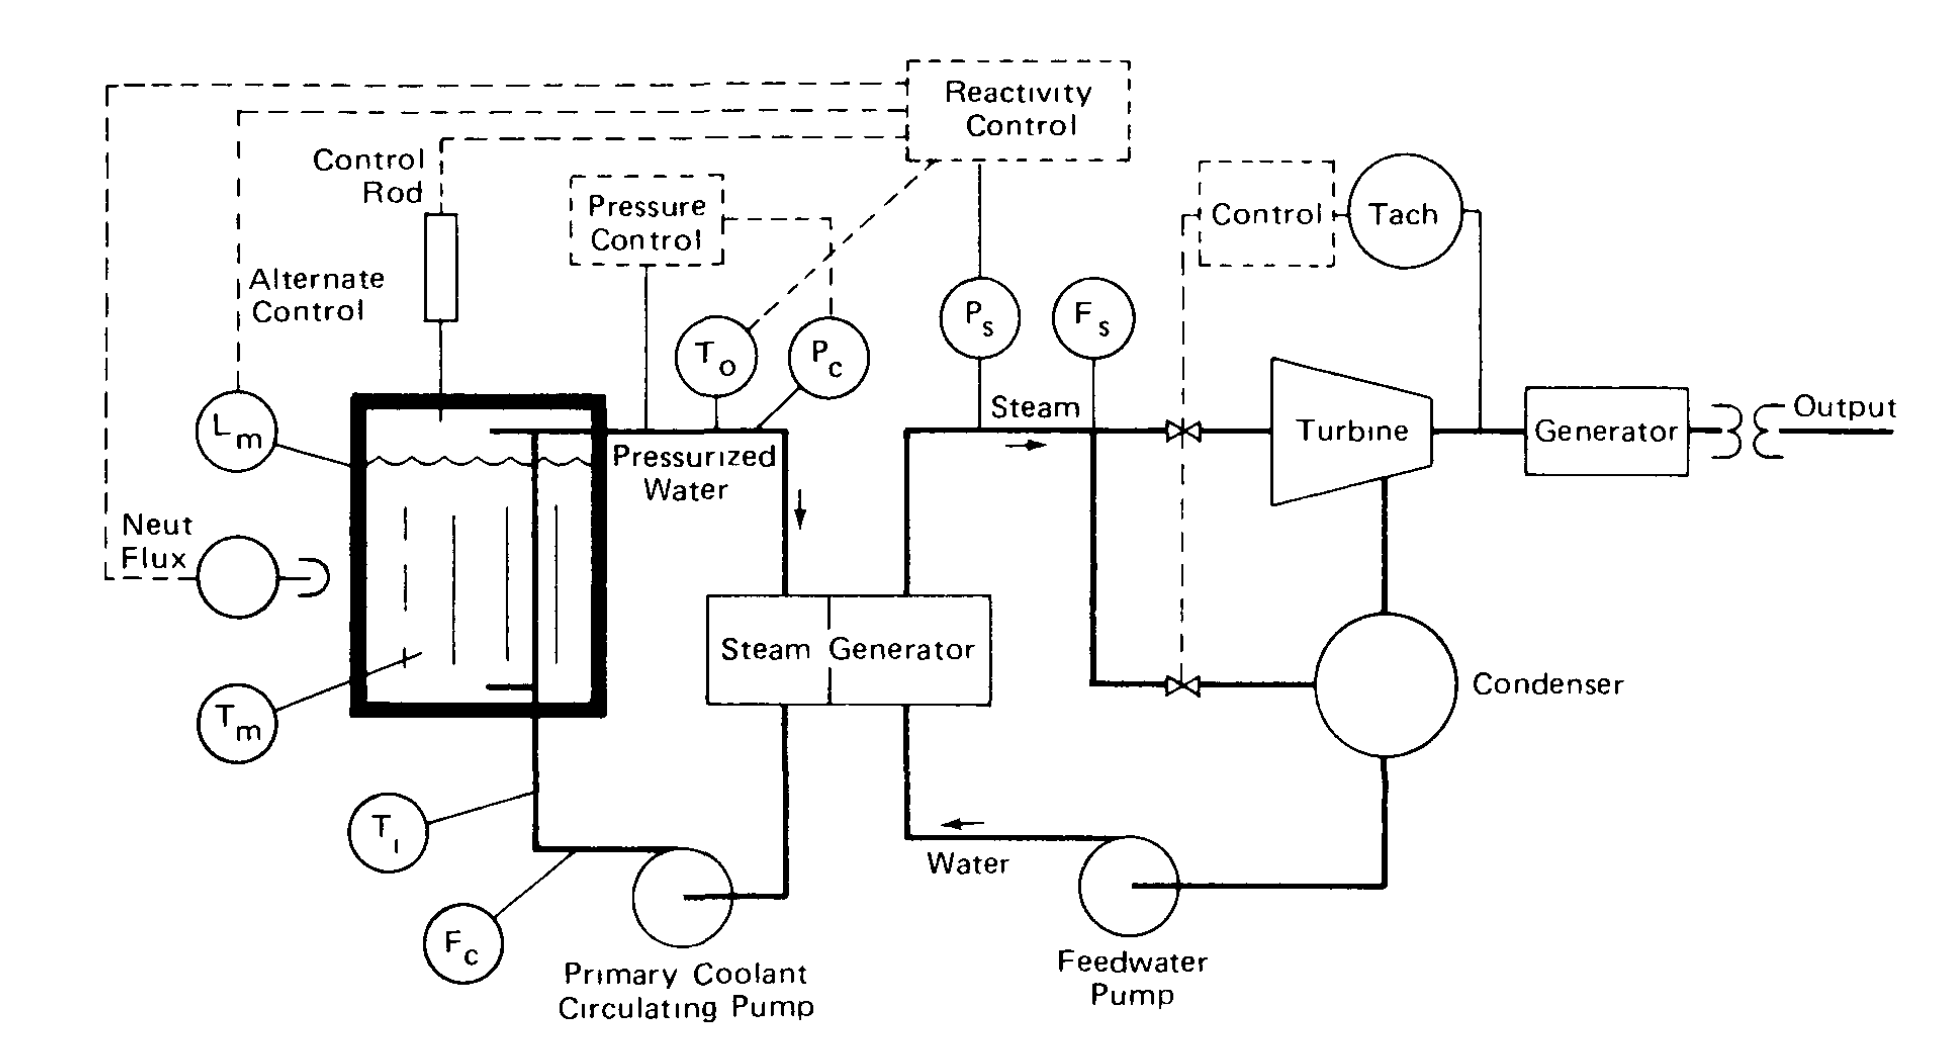
\includegraphics[width=0.8\textwidth]{instrumentation.png}
  \note{PWRs are the most common worldwide. Sensors track neutron flux, coolant temperature, rod position, pressure, and flow rate.}
\end{frame}

\begin{frame}{Automatic Protection Systems}
  \subsubsection*{SCRAMs and Interlocks}
  \note{Even the best operator can’t always react fast enough. That’s where automatic systems step in. SCRAMs instantly insert control rods. Protection logic compares real-time data to safety limits, triggering shutdowns, alarms, or backup actuation.}
  \begin{itemize}
    \item Reactor protection systems (RPS): monitor reactivity, temperature, pressure
    \item Logic interlocks: prevent unsafe configurations
    \item Hardwired paths with digital backups
  \end{itemize}
\end{frame}
\begin{frame}{Control Logic}
  \centering
  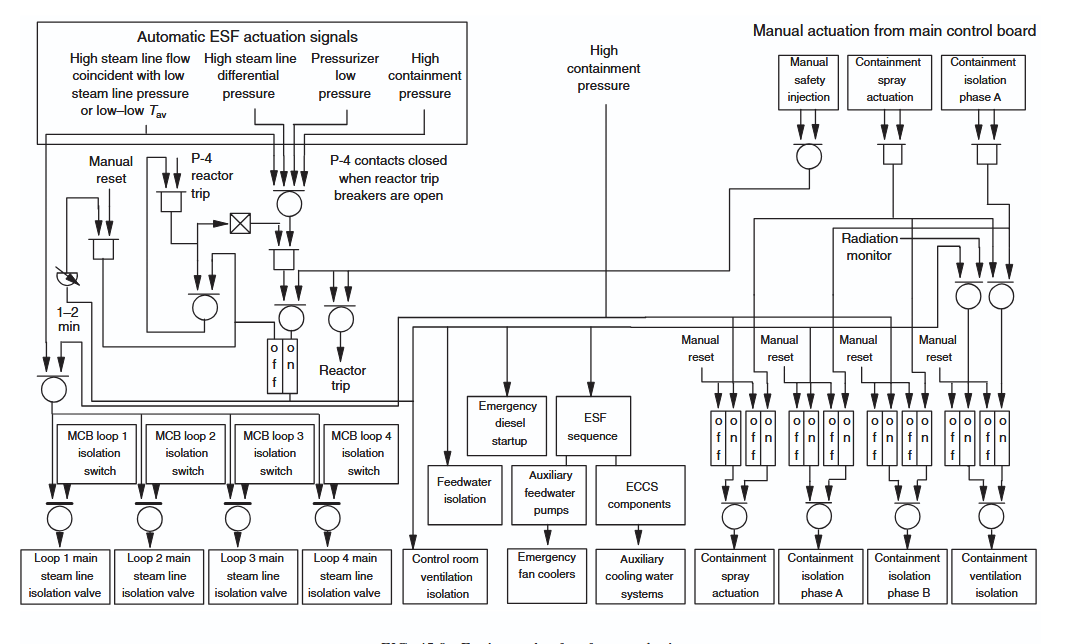
\includegraphics[width=0.95\textwidth]{safetylogic}
\end{frame}

\section{Historical Accidents}

\begin{frame}{SL-1: Prompt Critical Accident}
  \centering
  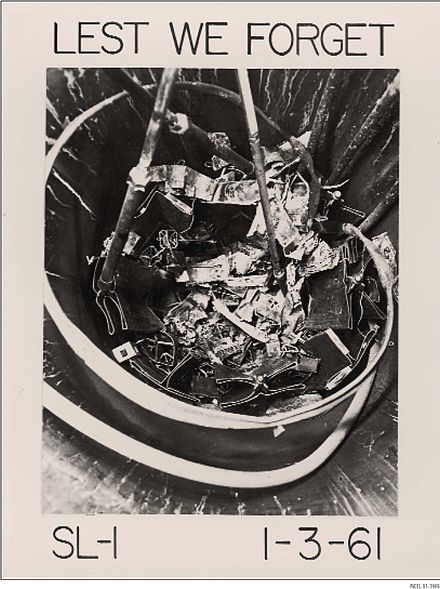
\includegraphics[width=0.4\textwidth]{sl1diagram.jpg}
  \note{Local firefighters arrived in response to a fire alarm and found the facility abandoned.
Coffee cups remained warm, and food was left uneaten. As radiation alarms activated on their
dosimetry equipment, they realized a serious radiological event had occurred. Two operators
were located dead from radiation exposure. The third, Richard Legg, was discovered impaled
and pinned to the containment ceiling by a control rod—ejected upward during the reactor’s
prompt critical event.}
\end{frame}

\begin{frame}{SL-1: Prompt Critical Accident}
  \begin{itemize}
    \item Occurred January 3, 1961 in Idaho Falls.
    \item A single control rod was withdrawn manually beyond safe limits.
    \item Caused an instantaneous power excursion and steam explosion.
    \item All three operators died; first fatal U.S. nuclear accident.
  \end{itemize}
  \note{Despite repeated reports of sticking rods, the system lacked mechanical or procedural
interlocks to prevent rapid withdrawal. A single operator retained full manual control, with
no redundancy or supervisory lockouts. The SL-1 event shows the critical role of human
factors engineering, particularly in minimizing design interfaces that allow unsafe manual
operations}
\end{frame}

\begin{frame}{Three Mile Island: Partial Core Meltdown}
  \centering
  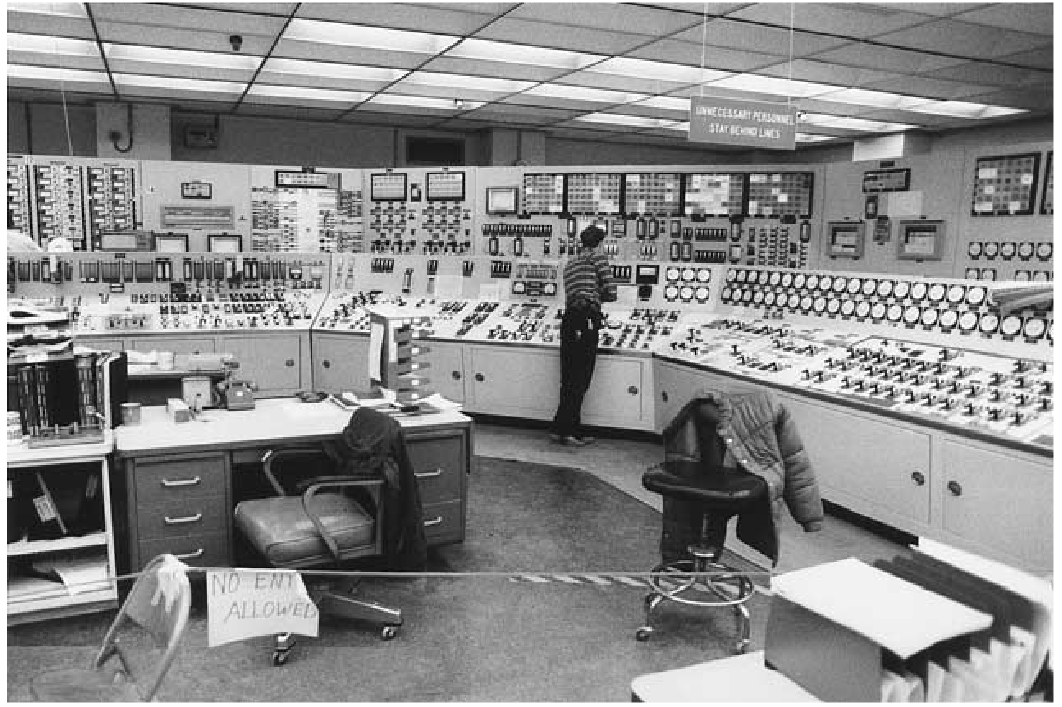
\includegraphics[width=0.75\textwidth]{tmicontrolroom.png}
  \note{The Three Mile Island Unit 2 (TMI-2) accident occurred on March 28, 1979, near Harrisburg,
Pennsylvania, and remains the most serious commercial nuclear accident in the United States.
It was precipitated by the failure of a pressure-operated relief valve (PORV) that became
stuck open during a minor malfunction. The valve allowed coolant to escape from the
pressurizer, but due to inadequate instrumentation, operators believed it had closed properly}
\end{frame}

\begin{frame}{Three Mile Island: Partial Core Meltdown}
  \begin{itemize}
    \item March 28, 1979 in Pennsylvania.
    \item Equipment failure: relief valve stuck open.
    \item Operator misinterpretation led to coolant pump shutdown.
    \item Reactor overheated—partial meltdown of core.
  \end{itemize}
  \note{Prior to this event, the relationship between human performance and system design was
underappreciated in reactor control engineering. It was often assumed that proper training
and “common sense” would be sufficient for managing system faults. However, the TMI-
2 accident highlighted that even well-trained operators can make catastrophic errors when
systems are not designed to support human cognition under stress.
As a result of this accident, the field of human factors engineering gained legitimacy within
the nuclear industry. Organizational and industrial psychology—especially the study of
ergonomics and operator-centered design—emerged as crucial disciplines in instrumentation
and control system development [6]. Operators needed interfaces not merely for function, but
for situational awareness and decision-making under pressure. This marked a turning point
in control room design philosophies, ushering in era-defining updates to alarm management,
display hierarchy, and interface logic}
\end{frame}

\begin{frame}{Chernobyl: Uncontrolled Power Surge}
  \centering
  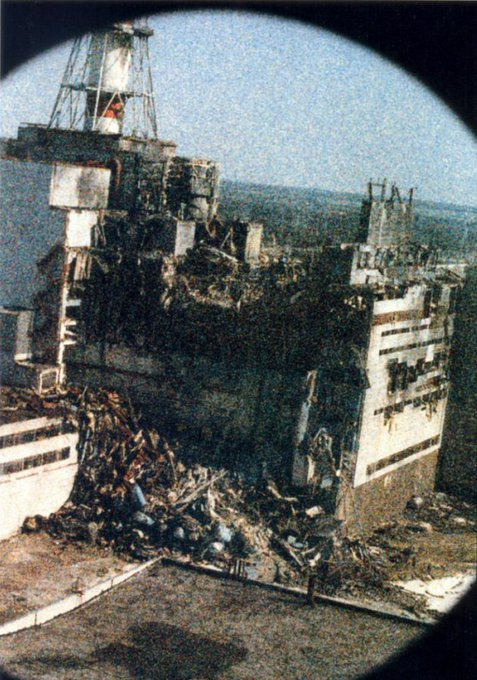
\includegraphics[width=0.65\textwidth]{chernobylafter.jpg}
  \note{The test intended to verify whether the rotational inertia
of the turbine could temporarily power the emergency coolant pumps in the event of a
grid power failure [7]. The RBMK-1000 reactor involved was a Soviet-designed graphite-
moderated, water-cooled system—flawed by both design and execution}
\end{frame}

\begin{frame}{Chernobyl: Uncontrolled Power Surge}
  \begin{itemize}
    \item April 26, 1986 in Pripyat, USSR.
    \item Unsafe test conducted at low power with flawed RBMK reactor.
    \item Positive void coefficient caused rapid reactivity increase.
    \item Control rods exacerbated the surge due to graphite tips.
    \item Reactor exploded; massive radioactive release.
  \end{itemize}
  \note{The core overheated instantly, rupturing fuel channels and vaporizing coolant. A vi-
olent steam explosion lifted the reactor’s 2,000-ton upper biological shield. A second ex-
plosion—possibly from hydrogen or steam—further breached the structure and exposed the
graphite moderator, which caught fire. Figure 6 shows the aftermath of the explosion mere
hours after the explosion. The fire lofted radioactive particles into the upper atmosphere,
affecting much of Europe }
\end{frame}

\begin{frame}
  \centering
  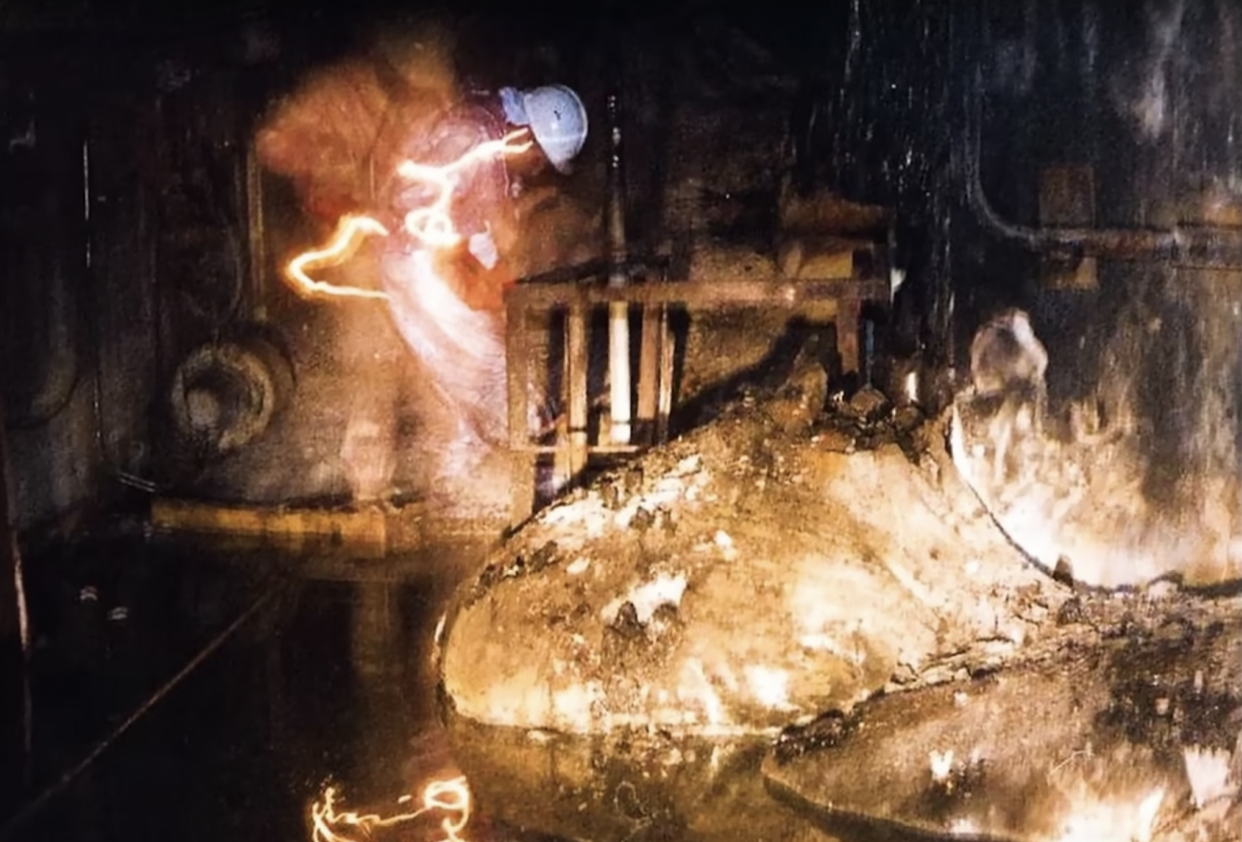
\includegraphics[width=0.65\textwidth]{elephantsfoot.png}
  \note{The aftermath of Chernobyl catalyzed global reevaluation of nuclear safety, reactor de-
sign, and operator training. The international community pushed for increased transparency,
safety audits, and enhanced containment strategies. The photograph in Figure 7 famously
shows the “Elephant’s Foot,” a deadly corium formation. The strange visual static in the
image is not lightning, but film degradation from intense radiation—testament to the un-
precedented radioactive environment at the site}
\end{frame}

\begin{frame}{Fukushima Daiichi: Station Blackout}
  \begin{itemize}
    \item March 11, 2011 in Japan.
    \item Magnitude 9.0 earthquake triggered tsunami.
    \item Backup diesel generators flooded—loss of core cooling.
    \item Hydrogen buildup led to explosions in three reactors.
  \end{itemize}
  \note{The Fukushima-Daiichi Nuclear Power Station, operated by TEPCO, was critically
affected. Although the three operating reactors—Units 1, 2, and 3—successfully SCRAMed
(shut down automatically), the tsunami flooded the site and disabled both the offsite grid
connections and emergency diesel generators [12]. This unprecedented loss of power across all
units is illustrated in Figure 8, which shows the reactor buildings after successive hydrogen
explosions.}
\end{frame}

\begin{frame}
  \centering
  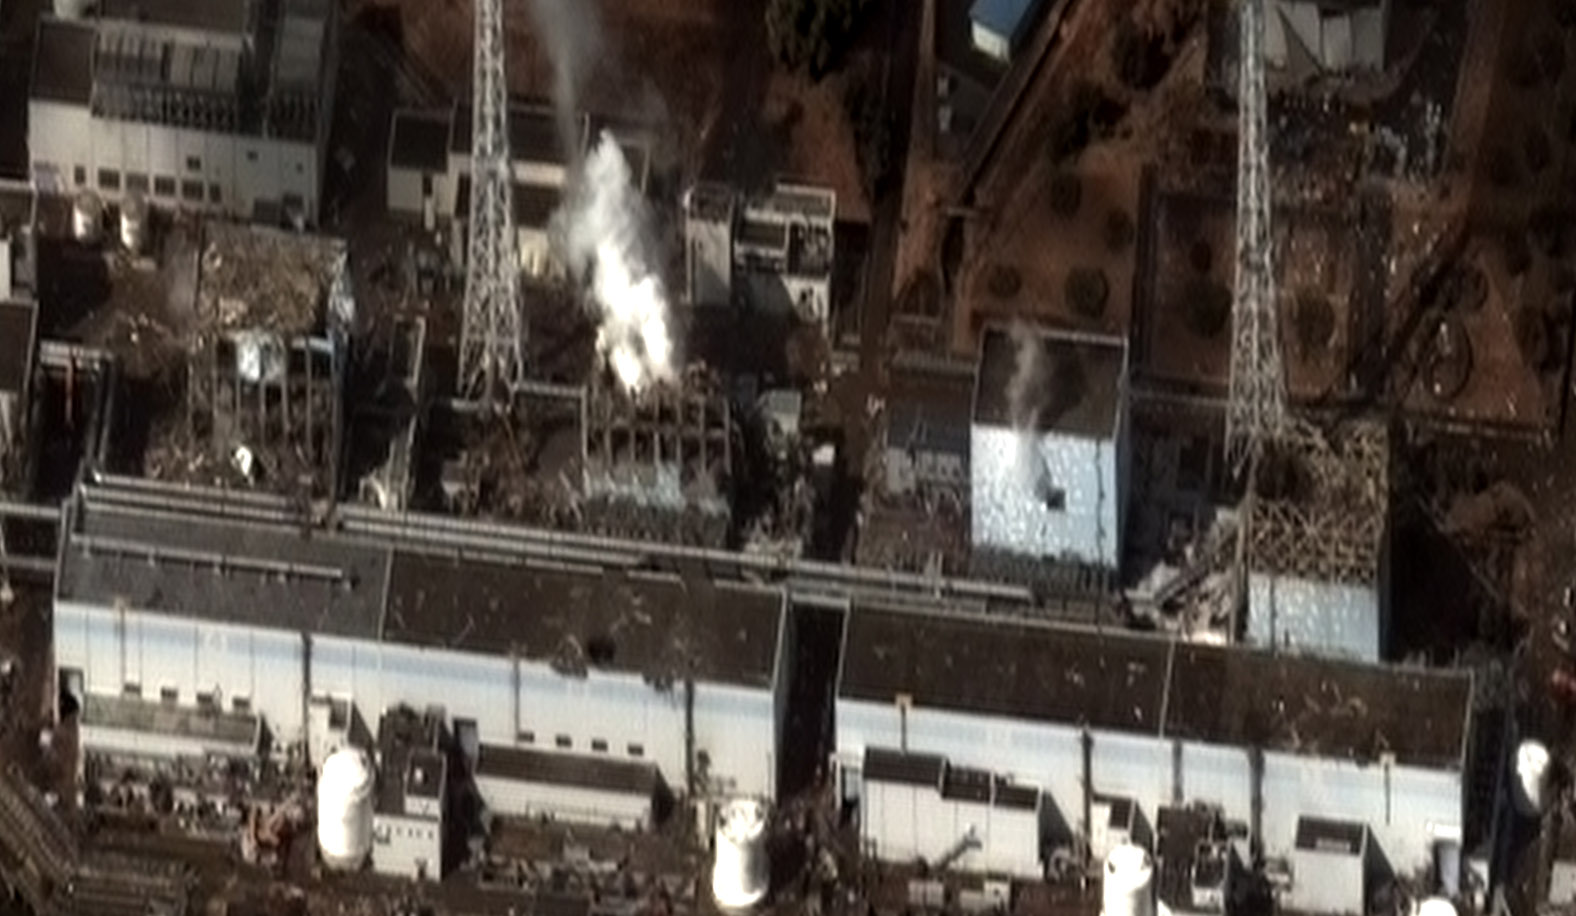
\includegraphics[width=\textwidth]{fukushimaafter.jpg}
  \note{Operators at Fukushima recognized the danger but were rendered effectively blind by
the loss of power. Unlike U.S. Navy reactor systems—where portable test equipment such
as Fluke digital multimeters can be attached to terminals for passive thermocouple read-
ings—the Fukushima design lacked redundant manual monitoring options. In a desperate
act of ingenuity, personnel retrieved car batteries from nearby vehicles and wired them in
series to restore minimal voltage to power essential instrumentation. Unfortunately, by the
time this improvised power source was implemented, core damage in Units 1, 2, and 3 was
already underway, with partial or full meltdown confirmed in post-event analyses}
\end{frame}

\section{Human and Ethical Design}

\begin{frame}{Human Operators: Essential Links}
  \centering
  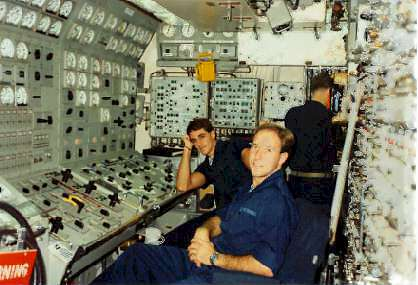
\includegraphics[width=0.75\textwidth]{maneuvering-watch.jpg}
  \note{}
\end{frame}

\begin{frame}{Human Operators: Essential Links}
  \begin{itemize}
    \item Human error was central to SL-1, TMI, and Chernobyl.
    \item Operators are responsible for interpreting ambiguous or conflicting signals.
    \item Training, vigilance, and mental workload matter.
  \end{itemize}
  \note{Despite automation, human judgment determines plant safety. Accidents often trace back to either misinterpretation or improper training.}
\end{frame}


\begin{frame}{Human Factors Engineering}
  \begin{itemize}
    \item Post-TMI, HFE became a formal discipline in nuclear plant design.
    \item Goals: reduce confusion, prevent overload, clarify alarms.
    \item INPO and NRC led redesigns of control interfaces.
  \end{itemize}
  \note{Human-machine interface redesign became essential after TMI. Alarm logic, indicator layout, and system feedback were all reengineered.}
\end{frame}

\begin{frame}{Operator Training}
  \centering
  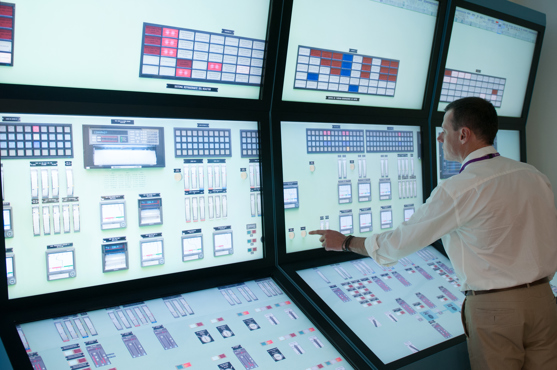
\includegraphics[width=0.75\textwidth]{simulators.jpg}
\end{frame}

\begin{frame}{Operator Training}
  \begin{itemize}
    \item U.S. Navy trains operators with year-long theoretical and practical curriculum.
    \item Qualification cards enforce step-by-step system mastery.
    \item Real-time simulators mimic full plant behavior—including failures.
  \end{itemize}
  \note{Simulators allow safe repetition of emergency scenarios. This procedural rigor is unmatched in civilian sectors.}
\end{frame}

\begin{frame}{Ethical Oversight in Automation}
  \centering
  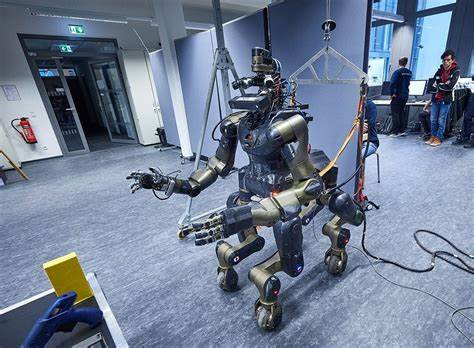
\includegraphics[width=0.65\textwidth]{ethicaldesign.jpg}
\end{frame}

\begin{frame}{Ethical Oversight in Automation}
  \begin{itemize}
    \item Systems must support—not replace—human oversight.
    \item Overreliance on automation can erode accountability.
    \item Ethical design considers failure modes, transparency, and operator input.
  \end{itemize}
  \note{Designing for ethical oversight means respecting human limits while reinforcing responsibility. The worst outcomes often arise when operators are sidelined.}
\end{frame}

\section{The Road Ahead}

\begin{frame}{Why Nuclear Declined}
  \subsubsection*{Policy, Perception, and Paralysis}
  \begin{itemize}
    \item Each accident—from SL-1 to Fukushima—prompted strict new regulations.
    \item Longer licensing cycles delayed new builds by decades.
    \item Public opposition and fear, not technical failure, stalled the industry.
    \item Skilled labor and supply chains diminished as construction halted.
  \end{itemize}
  \note{The world walked away not because nuclear failed—but because faith in its management eroded. Regulation became slower, and expertise drifted away.}
\end{frame}

\begin{frame}{Challenges Today}
  \begin{itemize}
    \item Most operating reactors in the U.S. are past mid-life.
    \item Replacing the aging nuclear workforce is a growing challenge.
    \item Engineering firms that once supported nuclear have pivoted to renewables.
    \item Safety margins remain—but the supporting infrastructure has weakened.
  \end{itemize}
  \note{Many of the companies and capabilities that built the first generation of plants no longer exist in their original form.}
\end{frame}

\section{Conclusion}

\begin{frame}{Conclusion: A Deliberate Future}
  \centering
  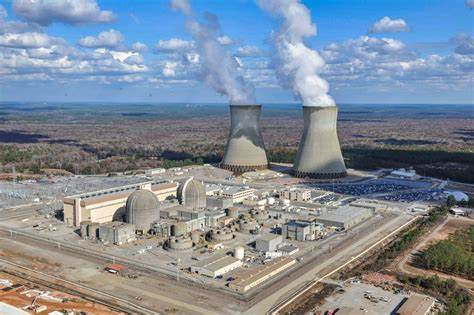
\includegraphics[width=0.55\textwidth]{vogtle}
\end{frame}

\begin{frame}{Conclusion: A Deliberate Future}
  \begin{itemize}
    \item Nuclear safety is engineered, not assumed.
    \item Instrumentation and human oversight must evolve together.
    \item Ethical design puts operators in control, not out of the loop.
    \item The tools are available—what remains is the will to rebuild trust.
  \end{itemize}
  \note{Safe nuclear power isn’t an inevitability—it’s a discipline. What matters is not just how reactors are built, but how they are overseen.}
\end{frame}

\end{document}
